\documentclass{article}

\usepackage{fancyhdr}
\usepackage{extramarks}
\usepackage{amsmath}
\usepackage{amsthm}
\usepackage{amsfonts}
\usepackage{tikz}
\usepackage{graphicx} %插入图片的宏包
\usepackage{float} %设置图片浮动位置的宏包
\usepackage{pythonhighlight}
% \usepackage{subfigure} %插入多图时用子图显示的宏包
% \usepackage[plain]{algorithm}
% \usepackage{algpseudocode}

% \usetikzlibrary{automata,positioning}

%
% Basic Document Settings
%

\topmargin=-0.45in
\evensidemargin=0in
\oddsidemargin=0in
\textwidth=6.5in
\textheight=9.0in
\headsep=0.25in

\linespread{1.1}

\pagestyle{fancy}
\lhead{\hmwkAuthorName}
\chead{\hmwkClass\ : \hmwkTitle}
\rhead{\firstxmark}
\lfoot{\lastxmark}
\cfoot{\thepage}

\renewcommand\headrulewidth{0.4pt}
\renewcommand\footrulewidth{0.4pt}

\setlength\parindent{0pt}


%代码格式设置



%
% Create Problem Sections
%

\newcommand{\enterProblemHeader}[1]{
    \nobreak\extramarks{}{Problem \arabic{#1} continued on next page\ldots}\nobreak{}
    \nobreak\extramarks{Problem \arabic{#1} (continued)}{Problem \arabic{#1} continued on next page\ldots}\nobreak{}
}

\newcommand{\exitProblemHeader}[1]{
    \nobreak\extramarks{Problem \arabic{#1} (continued)}{Problem \arabic{#1} continued on next page\ldots}\nobreak{}
    \stepcounter{#1}
    \nobreak\extramarks{Problem \arabic{#1}}{}\nobreak{}
}

\setcounter{secnumdepth}{0}
\newcounter{partCounter}
\newcounter{homeworkProblemCounter}
\setcounter{homeworkProblemCounter}{1}
\nobreak\extramarks{Problem \arabic{homeworkProblemCounter}}{}\nobreak{}

%
% Homework Problem Environment
%
% This environment takes an optional argument. When given, it will adjust the
% problem counter. This is useful for when the problems given for your
% assignment aren't sequential. See the last 3 problems of this template for an
% example.
%
\newenvironment{homeworkProblem}[1][-1]{
    \ifnum#1>0
        \setcounter{homeworkProblemCounter}{#1}
    \fi
    \section{Problem \arabic{homeworkProblemCounter}}
    \setcounter{partCounter}{1}
    \enterProblemHeader{homeworkProblemCounter}
}{
    \exitProblemHeader{homeworkProblemCounter}
}

%
% Homework Details
%   - Title
%   - Due date
%   - Class
%   - Section/Time
%   - Instructor
%   - Author
%

\newcommand{\hmwkTitle}{Quiz\ \#4}
\newcommand{\hmwkDueDate}{Dec 16, 2018}
\newcommand{\hmwkClass}{Complex Networks}
\newcommand{\hmwkClassTime}{Section A}
% \newcommand{\hmwkClassInstructor}{Professor Isaac Newton}
\newcommand{\hmwkAuthorName}{\textbf{RUOPENG XU} }
\newcommand{\hmwkAuthorNum}{\textbf{18M38179} }

%
% Title Page
%

\title{
    \vspace{2in}
    \textmd{\textbf{\hmwkClass:\ \hmwkTitle}}\\
    \normalsize\vspace{0.1in}\small{Due\ on\ \hmwkDueDate\ }\\
    % \vspace{0.1in}\large{\textit{\hmwkClassInstructor\ \hmwkClassTime}}
    \vspace{3in}
}

\author{\hmwkAuthorName\\ \hmwkAuthorNum}
\date{}

\renewcommand{\part}[1]{\textbf{\large Part \Alph{partCounter}}\stepcounter{partCounter}\\}

%
% Various Helper Commands
%

% Useful for algorithms
\newcommand{\alg}[1]{\textsc{\bfseries \footnotesize #1}}

% For derivatives
\newcommand{\deriv}[1]{\frac{\mathrm{d}}{\mathrm{d}x} (#1)}

% For partial derivatives
\newcommand{\pderiv}[2]{\frac{\partial}{\partial #1} (#2)}

% Integral dx
\newcommand{\dx}{\mathrm{d}x}

% Alias for the Solution section header
\newcommand{\solution}{\textbf{\large Solution}}

% Probability commands: Expectation, Variance, Covariance, Bias
\newcommand{\E}{\mathrm{E}}
\newcommand{\Var}{\mathrm{Var}}
\newcommand{\Cov}{\mathrm{Cov}}
\newcommand{\Bias}{\mathrm{Bias}}

\begin{document}

\maketitle

\pagebreak

\begin{homeworkProblem}
    % questions
What happens when a walker keeps walking for a long time on a graph?
\\
pi(t): probability that the walk is at vertex i at time t
\\
1. graph 1: find $AD^{-1}$

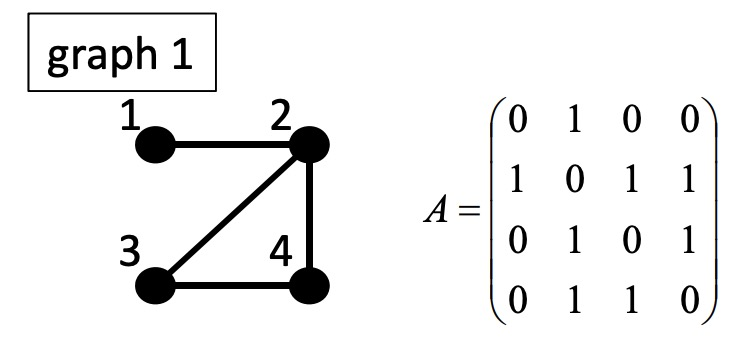
\includegraphics[scale=0.25]{quiz4_1.jpg}

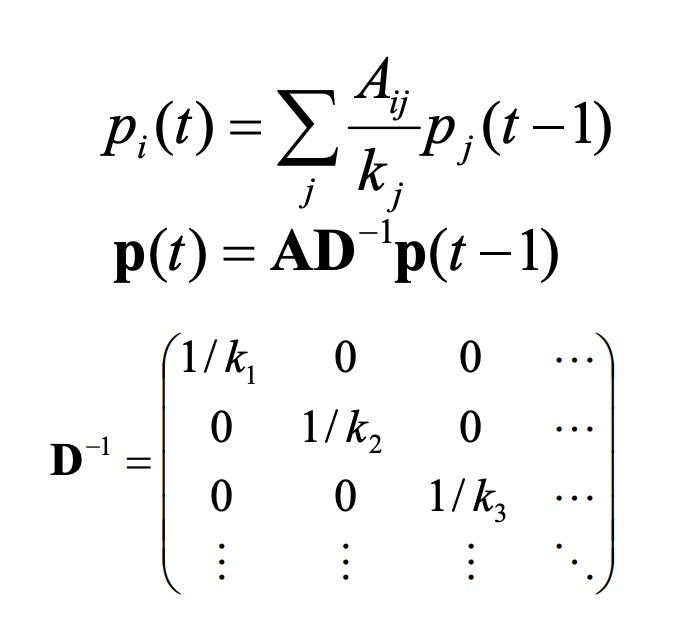
\includegraphics[scale=0.25]{quiz4_3.jpg}


\subsection*{Answer 1}
According to the defination of D
$D^{-1}$ = \\
$\displaystyle \begin{bmatrix}
1 & 0 & 0 & 0\\ 
0& \frac{1}{3} & 0 & 0 \\ 
0 & 0 & \frac{1}{2} & 0\\ 
0 & 0 & 0 & \frac{1}{2}
\end{bmatrix}$
\\
\\
Thus, $AD^{-1}$ = 
$ \displaystyle \begin{bmatrix}
0 & 1 & 0 & 0\\ 
1 & 0 & 1 & 1 \\ 
0 & 1 & 0 & 1\\ 
0 & 1 & 1 & 0
\end{bmatrix}$
$\times$
$ \displaystyle \begin{bmatrix}
1 & 0 & 0 & 0\\ 
0& \frac{1}{3} & 0 & 0 \\ 
0 & 0 & \frac{1}{2} & 0\\ 
0 & 0 & 0 & \frac{1}{2}
\end{bmatrix}$
=
$\begin{bmatrix}
0 & \frac{1}{3} & 0 & 0\\ 
1 & 0 & \frac{1}{2} & \frac{1}{2} \\ 
0 & \frac{1}{3} & 0 & \frac{1}{2}\\ 
0 & \frac{1}{3} & \frac{1}{2} & 0
\end{bmatrix}$





% \begin{python}

% \end{python}


\end{homeworkProblem}
\pagebreak

\begin{homeworkProblem}
2. graph 1: find p0(∞),p1(∞),p2(∞), and p3(∞)

\subsection*{Answer2}
When p -> ∞, the $p_{i}$(∞) is the probability of each node in the network.
According to the slides:

\textbf {probability is proportional to the degree of the vertex} and the sum of $p_{i}=1$
\\
Thus,
\\
\\
p0(∞)+p1(∞)+p2(∞)+p3(∞)=1,
\\
\\
make p0(∞)=x,p1(∞)=3x, p2(∞) = 2x,p3(∞) = 2x
\\
\\
x + 3x + 2x + 2x = 1
\\
\\
x = $\displaystyle \frac{1}{8}$
\\
\\
As a result,
$\displaystyle p0(\infty) = \frac{1}{8}, p1(\infty) = \frac{3}{8}, p2(\infty) = \frac{1}{4}, and, p3(\infty) = \frac{1}{4}$





\end{homeworkProblem}
\pagebreak




\begin{homeworkProblem}

3. graph 2: make a program of simulating random walks. show its results and answer the most visited node

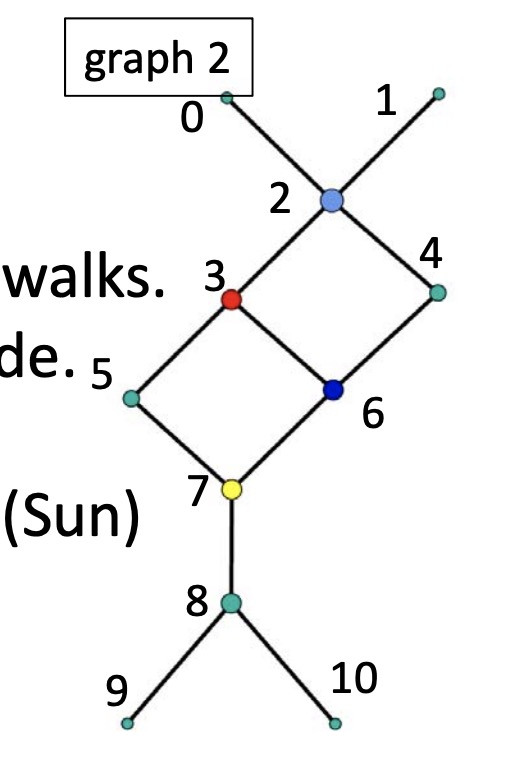
\includegraphics[scale=0.3]{quiz4_2.jpg}


\begin{python}
import networkx as nx
import matplotlib.pyplot as plt
import numpy as np

G = nx.Graph()
G.add_nodes_from(range(0,10))
G.add_edges_from([(0,2),(1,2),(2,3),(2,4),(3,5),(3,6),(4,6),(5,7),(6,7),(7,8),(8,9),(8,10)])
plt.figure(figsize=(5, 5))
nx.draw_spring(G, node_size=400, node_color='red', with_labels=True, font_weight='bold')
A = nx.adjacency_matrix(G).todense()
A = np.array(A, dtype = np.float64)
c = np.array([0, 0, 0, 0, 0, 0, 0, 0, 0, 0, 0]) # counter
walkLength = 100000 # random walk length
id = 0 # starting node (0-th)
for k in range(walkLength):
  p = A[id,:]
  id = np.random.choice(np.flatnonzero(p == p.max())) # random choice
  visited.append(id)
  c[id] = c[id] + 1
print(c)
\end{python}

Simulate we travel 10000 steps and try three times, according to the result:
\begin{python}
[ 4201  4289 16858 12600  8252  8285 12502 12453 12355  4045  4160]

[ 4294  4243 16836 12526  8287  8275 12580 12508 12309  4046  4096]

[ 4006  4100 16334 12456  8280  8425 12401 12572 12840  4282  4304]

\end{python}
Thus, the most visited node is node 2


\end{homeworkProblem}
\pagebreak





\end{document}
%
% Non sequential homework problems
%

% Jump to problem 18
